
\chapter{Descrição técnica dos sistemas}
\label{descricao_tecnica_dos_sistemas}

\section{Resumo da Especificação de requisitos}
Com a aplicação do sistema ePadaria vai se promover e otimizar a comunicação e funcionamento dos 3 setores, pedidos, cozinha e entregas.\\
Na gestão de pedidos, o gestor de pedidos, só terá que preencher dados na aplicação ePadaria, esta que trata de comunicar e verificar os stocks e também pedidos anteriores, que certifica que haverá espaço para o pedido no dia alocado, e dando ao gestor de pedidos imediatamente uma validação do pedido ou
refere o que estava invalido no pedido.\\
Na gestão de pedidos, o gestor de pedidos, só terá que preencher dados na aplicação ePadaria, esta que trata de comunicar e verificar os stocks e também pedidos anteriores, que certifica que haverá espaço para o pedido no dia alocado, e dando ao gestor de pedidos imediatamente uma validação do pedido ou refere o que estava invalido no pedido.\\


\section{Descrição do software que será necessário desenvolver}
\subsection{Requisitos funcionais}
\subsubsection{Casos de uso}
Na figura abaixo representa-se o modelo genérico de casos de uso do sistema ePadaria sob a forma de um diagrama de pacotes. Cada pacote agrega uma ou mais partes do sistema que se destinam a suportar processos da organização e/ou a reunir um conjunto de funcionalidades. Em cada pacote incluem-se alguns exemplos de Atores e casos de uso desenvolvidos para o sistema.

\begin{figure}[H]
	\centering
	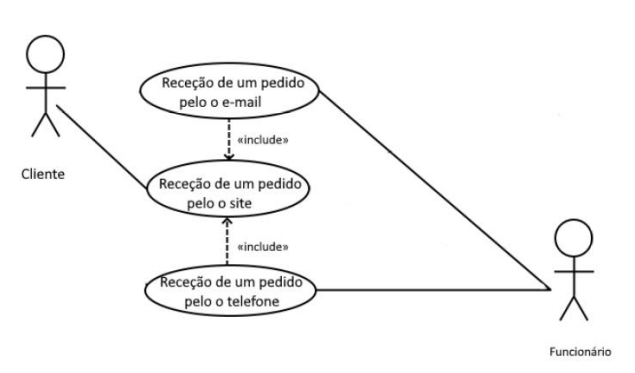
\includegraphics{diagrama_casos_de_uso}
	\caption{Diagrama de casos de uso}
	\label{fig:diagramacasosdeuso}
\end{figure}

\subsubsection{Requisitos}
Lista de requisitos para o caso de uso Receção de um pedido feito no site\\
\begin{figure}[H]
	\centering
	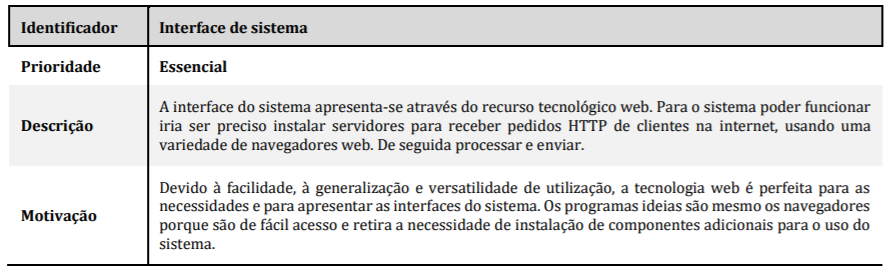
\includegraphics[width=15cm]{requisito_funcional1}
	\caption{Requisito funcional Interface do sistema}
	\label{fig:requisitofuncional1}
\end{figure}

\begin{figure}[H]
	\centering
	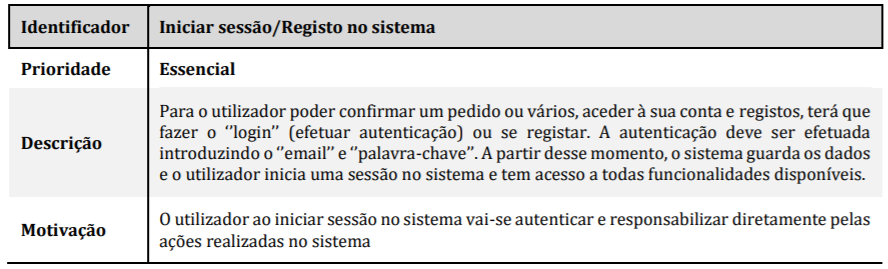
\includegraphics[width=15cm]{requisito_funcional2}
	\caption{Requisito funcional Iniciar Sessão/Registo no sistema}
	\label{fig:requisitofuncional2}
\end{figure}

\begin{figure}[H]
	\centering
	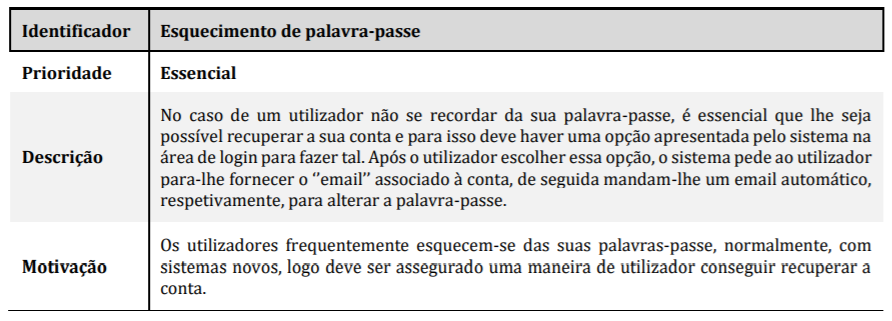
\includegraphics[width=15cm]{requisito_funcional3}
	\caption{Requisito funcional Esquecimento da palavra-passe}
	\label{fig:requisitofuncional3}
\end{figure}

\begin{figure}[H]
	\centering
	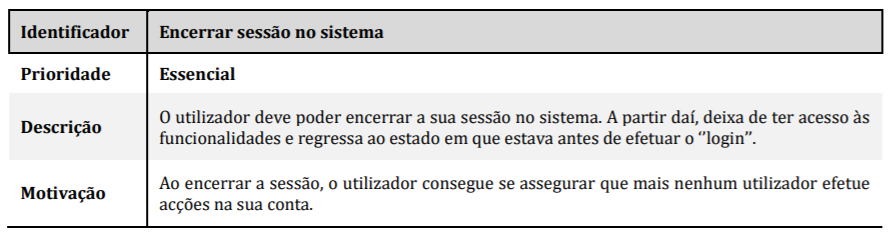
\includegraphics[width=15cm]{requisito_funcional4}
	\caption{Requisito funcional Encerrar sessão no sistema}
	\label{fig:requisitofuncional4}
\end{figure}

Lista de requisitos para o caso de uso Receção de um pedido efetuado por telefone\\

\begin{figure}[H]
	\centering
	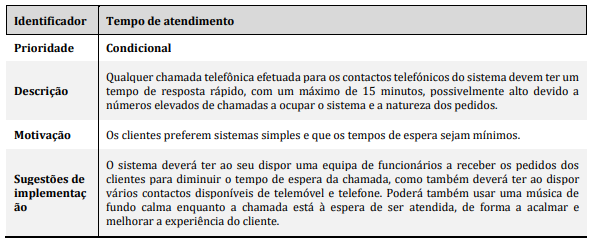
\includegraphics[width=15cm]{requisitofuncional5}
	\caption{Requisito funcional tempo de atendimento}
	\label{fig:requisitofuncional5}
\end{figure}

\begin{figure}[H]
	\centering
	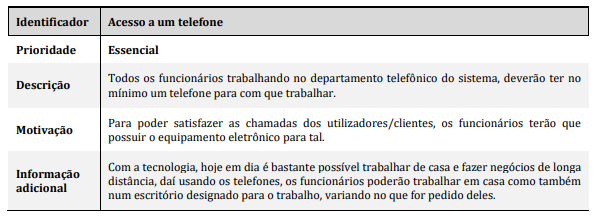
\includegraphics[width=15cm]{requisitofuncional6}
	\caption{Requisito funcional acesso a um telefone}
	\label{fig:requisitofuncional6}
\end{figure}



\begin{figure}[H]
	\centering
	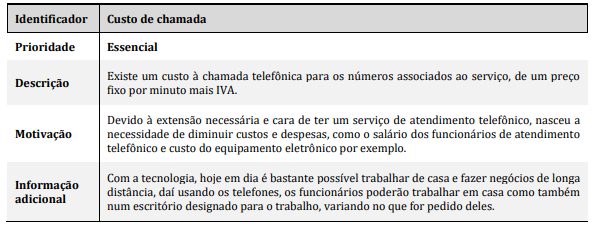
\includegraphics[width=15cm]{requisitofuncional7}
	\caption{Requisito funcional custo de chamada}
	\label{fig:requisitofuncional7}
\end{figure}

Lista de requisitos para o caso de uso Receção de um pedido efetuado por e-mail\\

\begin{figure}[H]
	\centering
	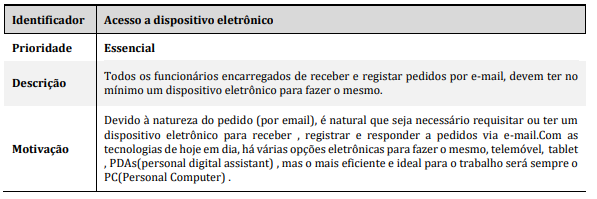
\includegraphics[width=15cm]{requisitofuncional8}
	\caption{Requisito funcional Acesso a dispositivo eletrónico}
	\label{fig:requisitofuncional8}
\end{figure}

\subsubsection{Requisitos não-funcionais}

\begin{figure}[H]
	\centering
	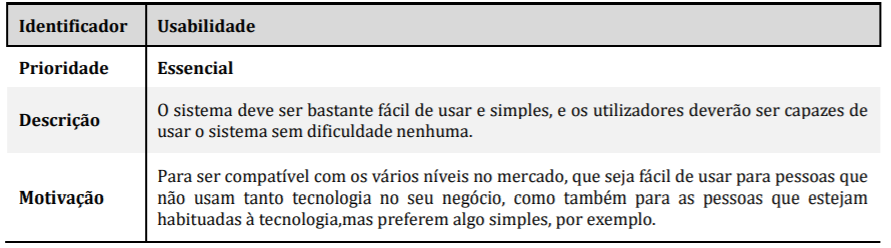
\includegraphics[width=15cm]{requisito_nao_funcional1}
	\caption{Requisito não funcional Usabilidade}
	\label{fig:requisitonaofuncional1}
\end{figure}

\begin{figure}[H]
	\centering
	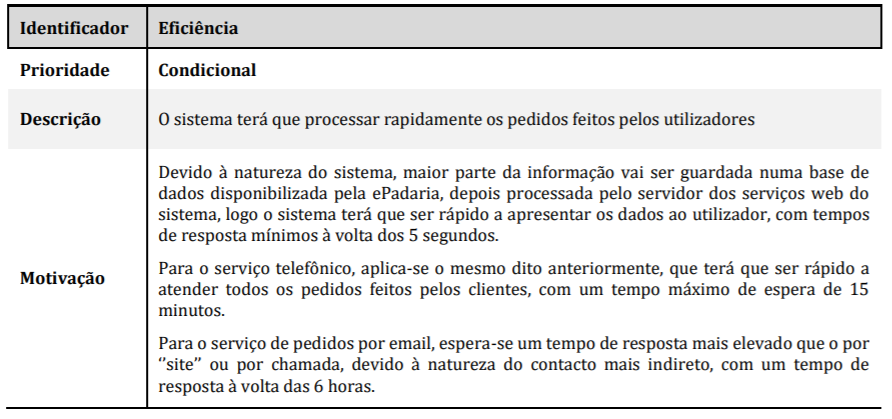
\includegraphics[width=15cm]{requisito_nao_funcional2}
	\caption{Requisito não funcional Eficiência}
	\label{fig:requisitonaofuncional2}
\end{figure}

\begin{figure}[H]
	\centering
	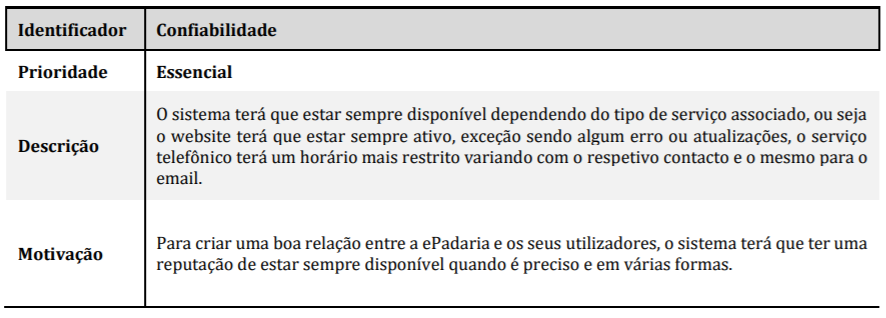
\includegraphics[width=15cm]{requisito_nao_funcional3}
	\caption{Requisito não funcional Confiabilidade}
	\label{fig:requisitonaofuncional3}
\end{figure}

\begin{figure}[H]
	\centering
	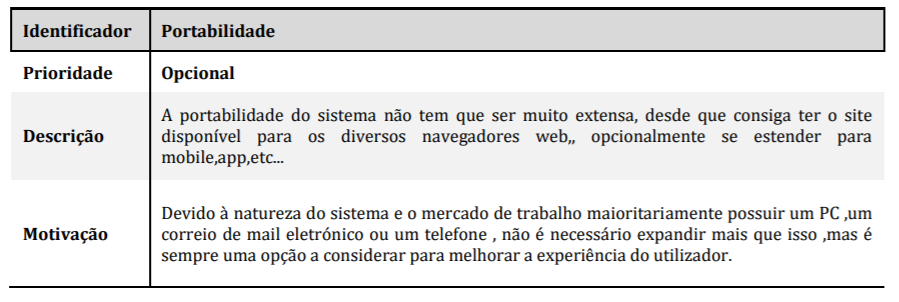
\includegraphics[width=15cm]{requisito_nao_funcional4}
	\caption{Requisito não funcional Portabilidade}
	\label{fig:requisitonaofuncional4}
\end{figure}

\begin{figure}[H]
	\centering
	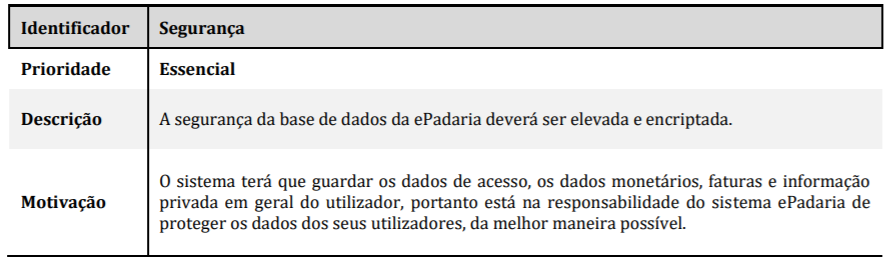
\includegraphics[width=15cm]{requisito_nao_funcional5}
	\caption{Requisito não funcional Segurança}
	\label{fig:requisitonaofuncional5}
\end{figure}

\begin{figure}[H]
	\centering
	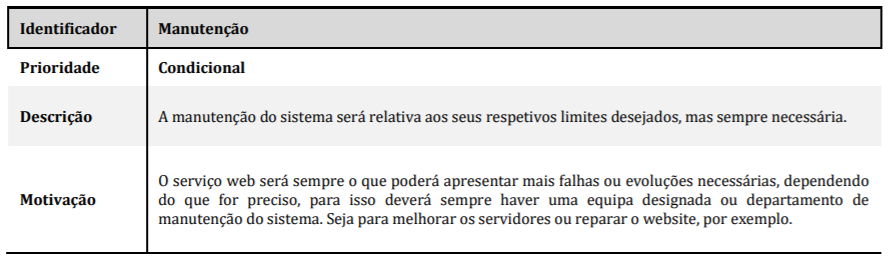
\includegraphics[width=15cm]{requisito_nao_funcional6}
	\caption{Requisito não funcional Manutençaõ}
	\label{fig:requisitonaofuncional6}
\end{figure}

\section{Descrição do estrutura física do hardware}
Para se poder usar o site será mais viavél o seu uso num computador ou tablet que em um telemóvel devido á sua estrutura e ter sido destinado mais para uso no computador. \\
Não é necessário se ter um dispositivo de alto desempenho para se poder aceder ao site e ser usado,apenas é necessário ter os requisitos minimos.\\
Por parte dos funcionários da padaria o melhor é usar algo e pelo menos médio desempenho de maneira a o sistema responder de forma rápida e não atrasar a produtividade.

Colocar diagrama de distribuição!!!!!!!!!!!!!!!!!!!!!!!!!!!!!
\section {Diagrama de Gantt}
\begin{figure}[H]
	\centering
	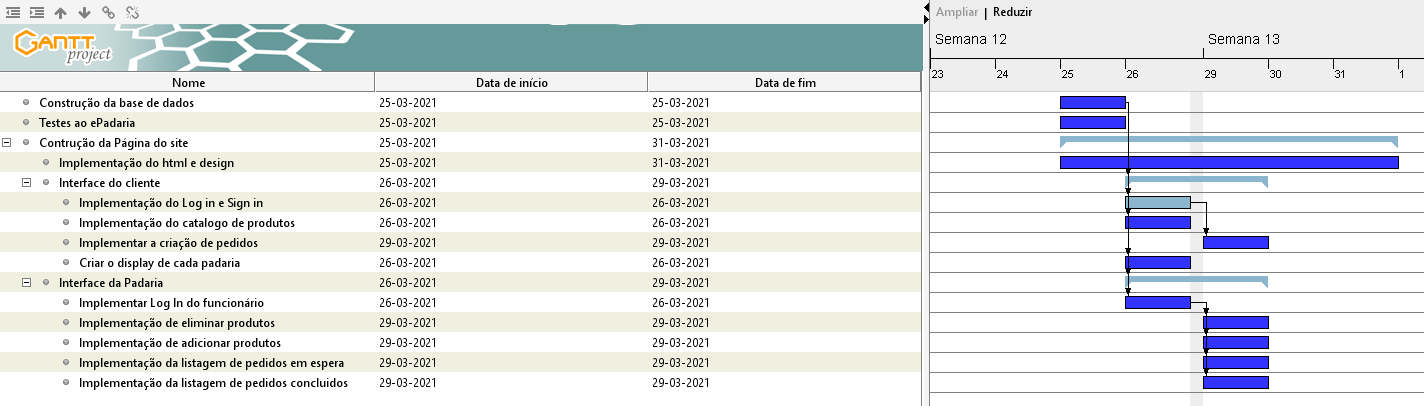
\includegraphics[width=6cm]{gantt}
	\caption{Gantt Poject do ePadaria}
	\label{fig:gantt}
\end{figure}




